\begin{figure}[ht]
    \centering

    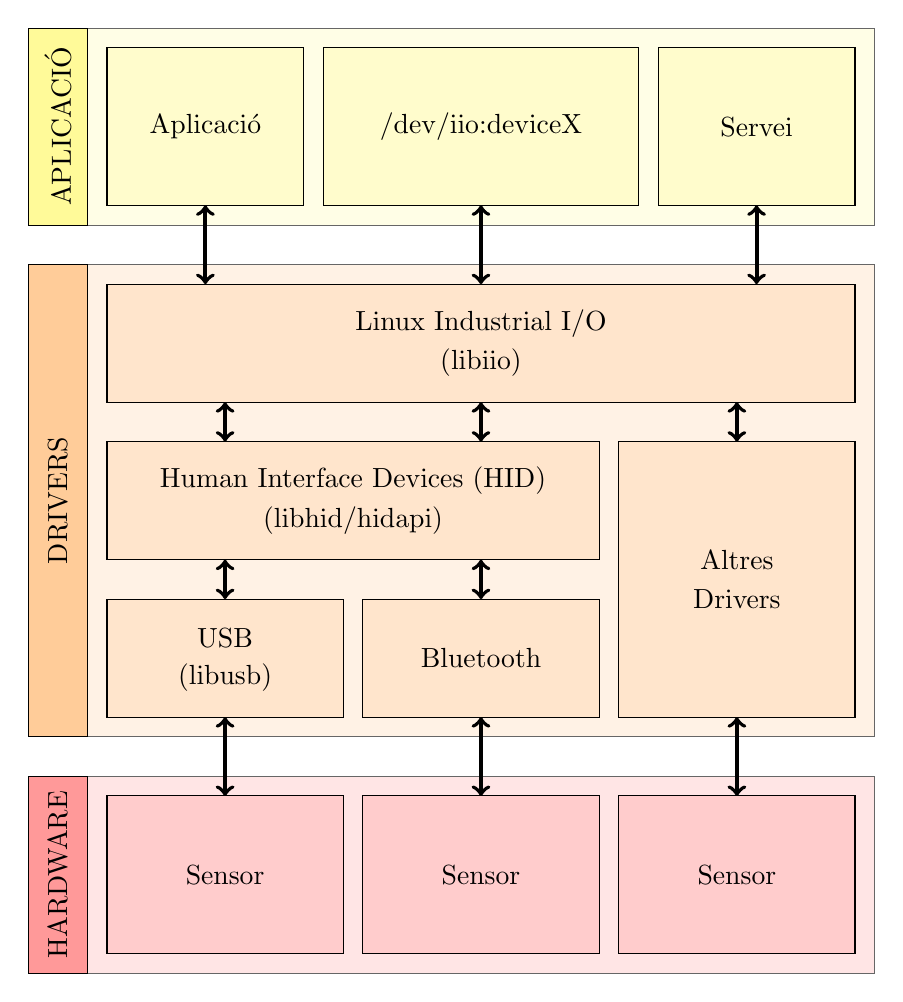
\begin{tikzpicture}
        \filldraw[fill=red!10!white, draw=black!60!white] (0.75,0) rectangle (10.75,2.5);
        \filldraw[fill=orange!10!white, draw=black!60!white] (0.75,3) rectangle (10.75,9);
        \filldraw[fill=yellow!10!white, draw=black!60!white] (0.75,9.5) rectangle (10.75,12);
    
        \filldraw[fill=red!40!white, draw=black] (0,0) rectangle (0.75,2.5);
        \filldraw[fill=orange!40!white, draw=black] (0,3) rectangle (0.75,9);
        \filldraw[fill=yellow!40!white, draw=black] (0,9.5) rectangle (0.75,12);
    
        \node at (0.375,1.25) {\rotatebox{90}{HARDWARE}};
        \node at (0.375,6) {\rotatebox{90}{DRIVERS}};
        \node at (0.375,10.75) {\rotatebox{90}{APLICACIÓ}};
    
        \filldraw[fill=red!20!white, draw=black] (1,0.25) rectangle (4,2.25);
        \node at (2.5,1.25) {Sensor};
        \filldraw[fill=red!20!white, draw=black] (4.25,0.25) rectangle (7.25,2.25);
        \node at (5.75,1.25) {Sensor};
        \filldraw[fill=red!20!white, draw=black] (7.5,0.25) rectangle (10.5,2.25);
        \node at (9,1.25) {Sensor};
    
        \filldraw[fill=orange!20!white, draw=black] (1,3.25) rectangle (4,4.75);
        \node at (2.5,4.25) {USB};
        \node at (2.5,3.75) {(\fitx{libusb})};
        \filldraw[fill=orange!20!white, draw=black] (4.25,3.25) rectangle (7.25,4.75);
        \node at (5.75,4) {Bluetooth};
        \filldraw[fill=orange!20!white, draw=black] (1,5.25) rectangle (7.25,6.75);
        \node at (4.125,6.25) {Human Interface Devices (HID)};
        \node at (4.125,5.75) {(\fitx{libhid}/\fitx{hidapi})};
    
        \filldraw[fill=orange!20!white, draw=black] (7.5,3.25) rectangle (10.5,6.75);
        \node at (9,5.25) {Altres};
        \node at (9,4.75) {Drivers};
        \filldraw[fill=orange!20!white, draw=black] (1,7.25) rectangle (10.5,8.75);
        \node at (5.75,8.25) {Linux Industrial I/O};
        \node at (5.75,7.75) {(\fitx{libiio})};
    
        \filldraw[fill=yellow!20!white, draw=black] (1,9.75) rectangle (3.5,11.75);
        \node at (2.25,10.75) {Aplicació};
        \filldraw[fill=yellow!20!white, draw=black] (3.75,9.75) rectangle (7.75,11.75);
        \node at (5.75,10.75) {\fitx{/dev/iio:deviceX}};
        \filldraw[fill=yellow!20!white, draw=black] (8,9.75) rectangle (10.5,11.75);
        \node at (9.25,10.75) {Servei};
    
        \draw[line width=0.5mm, <->] (2.5,2.25) -- (2.5,3.25);
        \draw[line width=0.5mm, <->] (5.75,2.25) -- (5.75,3.25);
        \draw[line width=0.5mm, <->] (9,2.25) -- (9,3.25);
    
        \draw[line width=0.5mm, <->] (2.5,4.75) -- (2.5,5.25);
        \draw[line width=0.5mm, <->] (5.75,4.75) -- (5.75,5.25);
    
        \draw[line width=0.5mm, <->] (2.5,6.75) -- (2.5,7.25);
        \draw[line width=0.5mm, <->] (5.75,6.75) -- (5.75,7.25);
        \draw[line width=0.5mm, <->] (9,6.75) -- (9,7.25);
    
        \draw[line width=0.5mm, <->] (2.25,8.75) -- (2.25,9.75);
        \draw[line width=0.5mm, <->] (5.75,8.75) -- (5.75,9.75);
        \draw[line width=0.5mm, <->] (9.25,8.75) -- (9.25,9.75);
    
    \end{tikzpicture}

    \caption{Esquema de les capes d'abstracció per a un dispositiu \est{iio} a Linux.}
    \label{fig:linux-stack}
\end{figure}
